
\section{拓扑（与诺特）性质}

许多\trTopology{}概念，用到底\trTopologicalSpace{} $\Spec A$ 上、日后再用到\trScheme{}上，都很有用。

\textbf{3.6.1.\ $\Spec A$ 可能具有的\trTopology{}属性：\trConnected{}性、\trIrreducible{}性、\trQuasicompactness{}。}

\textbf{3.6.2.}\ \emph{\trConnected{}性。}\quad 若一个\trTopologicalSpace{}不能写成两个非空\trOpenSet{}的\trDisjointUnion，就称它是\textbf{\trConnected}（connected）的。\cref{ex:product-ring-homeomorphism} 给出一个不\trConnected{}的 $\Spec A$ 的例子，而其后的注记将解释：一切例子都是这种形式。

\begin{exercise}\label{ex:product-ring-homeomorphism}
设 $A=A_1\times A_2\times\cdots\times A_n$。描述一个\trHomeomorphism
\[
\Spec A_1\sqcup\Spec A_2\sqcup\cdots\sqcup\Spec A_n\longrightarrow\Spec A
\]
使得每个 $\Spec A_i$ 都被映满 $\Spec A$ 的一个\trDistinguishedOpen{} $D(f_i)$。于是，作为\trTopologicalSpace，$\Spec\prod_{i=1}^{n}A_i=\bigsqcup_{i=1}^{n}\Spec A_i$。（提示：为方便起见先化归到 $n=2$。令 $f_1=(1,0)$、$f_2=(0,1)$。）
\end{exercise}

\textbf{3.6.3.}\ \emph{注记：\trIdempotent{}-\trConnected{}性套餐。}\footnote{译注：「套餐」原文 \emph{package}，兼有「（软件）包」与「整套方案」之意。}\quad \cref{ex:product-ring-homeomorphism} 的一个推广是：$\Spec A$ 不\trConnected，当且仅当 $A$ 同构于两个非零\trRing{} $A_1$ 与 $A_2$ 的乘积。关键想法是证明这两个条件都等价于：存在非零的 $a_1,a_2\in A$ 使得 $a_1^2=a_1$、$a_2^2=a_2$、$a_1+a_2=1$，从而 $a_1a_2=0$。满足 $a^2=a$ 的元素 $a\in A$ 称为\textbf{\trIdempotent{}}（idempotent）。这将在练习~10.5.L 中出现。

\textbf{3.6.4.}\ \emph{\trIrreducible{}性。}\quad 称一个\trTopologicalSpace{}为\textbf{\trIrreducible}（irreducible）的，如果它非空，并且它不是两个真\trClosedSubset{}之并。换言之，非空\trTopologicalSpace{} $X$ 是\trIrreducible{}的，若只要 $X=Y\cup Z$（其中 $Y$ 与 $Z$ 在 $X$ 中闭），就有 $Y=X$ 或 $Z=X$。等价地（而且更有用）：$X$ 的任意两个非空\trOpenSubset{}都相交。在经典几何中这是一个用处较小的概念——$\mathbb{C}^2$ 是\emph{可约}的（reducible，即非\trIrreducible），但我们将会看到 $\mathbb{A}^2_{\mathbb{C}}$ 是\trIrreducible{}的（\cref{ex:integral-domain-irreducible}）。

\begin{exercise}[容易的练习]\label{ex:irreducible-open-dense}
(a)~证明：在\trIrreducible{}\trTopologicalSpace{}中，任何非空\trOpenSet{}都\trDense{}。（因此你将会看到：与\trClassicalTopology{}不同，在\trZariskiTopology{}中，非空\trOpenSet{}全都「巨大」。）

(b)~设 $X$ 是\trTopologicalSpace，$Z$ 是一个子集（带子空间拓扑），证明：$Z$ 是\trIrreducible{}的，当且仅当它在 $X$ 中的闭包 $\overline{Z}$ 是\trIrreducible{}的。
\end{exercise}

\begin{exercise}[容易的练习]\label{ex:integral-domain-irreducible}
设 $A$ 是\trIntegralDomain，证明 $\Spec A$ 是\trIrreducible{}的。（提示：留意\trGenericPoint{} $[(0)]$。）我们将在练习~3.7.G 中把它推广。
\end{exercise}

\begin{exercise}\label{ex:irreducible-connected}
证明\trIrreducible{}\trTopologicalSpace{}是\trConnected{}的。
\end{exercise}

\begin{exercise}\label{ex:connected-reducible-example}
给出（并证明！）一个\trRing{} $A$ 的例子，使得 $\Spec A$ \trConnected{}但可约。（可能的提示：一幅图也许有帮助。符号「$\times$」有两「块」，却又是\trConnected{}的。）
\end{exercise}

\begin{exercise}[棘手的练习]\label{ex:twisted-cubic-cone}
(a)~设 $I=(wz-xy,\,wy-x^2,\,xz-y^2)\subset k[w,x,y,z]$。证明 $\Spec k[w,x,y,z]/I$ 是\trIrreducible{}的，证明途径是：证 $k[w,x,y,z]/I$ 是\trIntegralDomain。（这很难，所以给出若干可能提示之一：证明 $k[w,x,y,z]/I$ 同构于 $k[a,b]$ 中由次数被 $3$ 整除的单项式生成的 $k$-子代数。也还有别的进路，其中一些我们日后会见到。这是一类困难问题的实例：你怎样判断一个理想是不是\trPrimeIdeal？）日后我们将看到它就是\emph{\trTwistedCubic{}}（twisted cubic curve）上的\trCone{}（该曲线定义于练习~9.3.A，而它又是\trVeronese{}嵌入（\S9.3.6）的一个特例）。

\hard\ (b)~注意 (a) 中那个理想的生成元可以改写成保证
\[
\operatorname{rank}\left(\begin{array}{ccc}
w & x & y \\
x & y & z
\end{array}\right)\le 1
\]
的诸方程，也就是说，改写成诸 $2\times 2$ 子矩阵的行列式。把 (a) 推广到秩一的 $2\times n$ 矩阵的理想。这一概念将对应于\emph{$n$ 次\trRationalNormalCurve{}}（rational normal curve）（练习~9.3.I）上的\trCone{}（\S9.3.11）。
\end{exercise}

\textbf{3.6.5.}\ \emph{\trQuasicompactness{}。}\quad 若一个\trTopologicalSpace{} $X$ 满足：给定任意由\trOpenSet{}构成的\trCover{} $X=\bigcup_{i\in I}U_i$，都存在\trIndexSet{} $I$ 的有限子集 $S$ 使得 $X=\bigcup_{i\in S}U_i$，就称 $X$ 是\textbf{\trQuasicompact}（quasicompact）的。非正式地说：每个\trOpenCover{}都有有限子覆盖。我们会喜欢上这个条件，因为我们惧怕无穷。视你对「\trCompactness」的定义而定，这就是\trCompactness{}的定义，只不过可能要减去一条\trHausdorff{}条件。然而，这并不是「\trCompact」在代数几何中的真正类比（我们当然不愿让 $\mathbb{A}^1_{\mathbb{C}}$ 是\trCompact{}的）——正确的类比是「\trProperness{}」（properness，\S11.4）。

\begin{exercise}\label{ex:spec-quasicompact}
(a)~证明 $\Spec A$ 是\trQuasicompact{}的。（提示：练习~3.5.C。）

\hard\ (b)~（较不重要）证明：一般地，$\Spec A$ 可以有非\trQuasicompact{}的\trOpenSet。可能的提示：令 $A=k[x_1,x_2,x_3,\dots]$，$\mathfrak{m}=(x_1,x_2,\dots)\subset A$，考虑 $V(\mathfrak{m})$ 的补集。这个例子日后对构造其他「反例」有用（例如练习~8.1.F 与练习~5.1.K）。在\cref{ex:noetherian-open-quasicompact} 中我们将看到，对「足够好」（\trNoetherian）的环，这种古怪行为并不会发生。
\end{exercise}

\begin{exercise}\label{ex:finite-union-quasicompact}
(a)~设\trTopologicalSpace{} $X$ 是有限多个\trQuasicompact{}空间之并，证明 $X$ 是\trQuasicompact{}的。

(b)~证明\trQuasicompact{}\trTopologicalSpace{}的每个\trClosedSubset{}都是\trQuasicompact{}的。
\end{exercise}

\textbf{3.6.6.}\ \extrahard\ \emph{有趣却不相干的注记。}\quad \cref{ex:product-ring-homeomorphism} 表明 $\bigsqcup_{i=1}^{n}\Spec A_i\cong\Spec\prod_{i=1}^{n}A_i$，但当「$n$ 无穷」且诸 $A_i$ 皆非零时，这\emph{绝不}成立，因为任何\trRing{}的谱都是\trQuasicompact{}的（\cref{ex:spec-quasicompact}(a)）。这引出一个有趣的现象。我们来证明：$\Spec\prod_{i=1}^{\infty}A_i$ 严格大于 $\bigsqcup_{i=1}^{\infty}\Spec A_i$（其中每个 $A_i$ 都同构于\trField{} $k$）。首先，作为集合有包含关系 $\bigsqcup_{i=1}^{\infty}\Spec A_i\hookrightarrow\Spec\prod_{i=1}^{\infty}A_i$，因为对每个 $i$，$\prod A_i$ 中都有一个\trMaximalIdeal{}与之对应（确切地说，由那些在第 $i$ 个分量中为 $0$ 的元素组成）。但 $\prod A_i$ 还有别的\trMaximalIdeal。提示：描述一个不含于这些\trMaximalIdeal{}中任何一个的\trProperIdeal。（一个想法：考虑「最终为零」的元素 $\prod a_i$，即对 $i\gg 0$ 有 $a_i=0$。）这引出\emph{\trUltrafilter{}}（ultrafilter）的概念，它非常有用，却与我们眼下的讨论不相干。

\textbf{3.6.7.\ $\Spec A$ 的点可能具有的\trTopology{}性质。}

\textbf{3.6.8.}\ \emph{\trhDefinition{}。}\quad 若\trTopologicalSpace{}的点 $p\in X$ 满足 $\{p\}$ 是\trClosedSubset，就称它是一个\textbf{\trClosedPoint}（closed point）。在 $\mathbb{C}^n$ 的\trClassicalTopology{}中，所有的点都是闭的。在 $\Spec\mathbb{Z}$ 与 $\Spec k[t]$ 中，除 $[(0)]$ 外，所有的点都是闭的。

\begin{exercise}\label{ex:closed-points-maximal-ideals}
证明 $\Spec A$ 的\trClosedPoint{}对应于诸\trMaximalIdeal。（特别地，非空\trAffineScheme{}\emph{拥有}\trClosedPoint，因为非零\trRing{}有\trMaximalIdeal，\S0.3。）
\end{exercise}

\textbf{3.6.9.}\ \emph{与经典\trVarietyTheory{}的联系。}\quad \trHilbert{}\trNullstellensatz{}让我们能把 $\mathbb{A}^n_{\mathbb{C}}$ 的\trClosedPoint{}解释为复数的 $n$ 元组。更一般地，$\Spec\overline{k}[x_1,\dots,x_n]/(f_1,\dots,f_r)$ 的\trClosedPoint（其中 $\overline{k}$ 是\trAlgClosedField）自然地被解释为 $\overline{k}^{\,n}$ 中满足方程 $f_1=\cdots=f_r=0$ 的那些点（例如见\cref{ex:quotient-primes-bijection} 与 \cref{ex:inclusion-quotient-localization}(a)）。于是从现在起，讨论 $\mathbb{A}^n_{\overline{k}}$ 的子集时，我们将说「\trClosedPoint」而不说「传统点」，说「非\trClosedPoint{}」而不说「附赠点」。下面的练习正是代数簇上\trClosedPoint{}之集为\trDense{}这一事实的缘由（参看练习~5.3.F 与定义~11.2.9）。

\begin{exercise}\label{ex:closed-points-dense}
(a)~设 $k$ 是\trField，$A$ 是有限生成的 $k$-代数。证明 $\Spec A$ 的\trClosedPoint{}之集是\trDense{}的；证明途径是：设 $f\in A$，而 $D(f)$ 是 $\Spec A$ 的一个非空（特异）\trOpenSubset，证明 $D(f)$ 含有 $\Spec A$ 的一个\trClosedPoint。提示：注意 $A_f$ \emph{也}是有限生成的 $k$-代数。用\trNullstellensatz（\cref{thm:hilbert-nullstellensatz}）来辨认有限生成 $k$-代数 $B$ 之谱的\trClosedPoint：即那些\trResidueField（$B$ 对相应\trMaximalIdeal{}的商）是 $k$ 的有限扩张的点。对 $B=A$ 与 $B=A_f$ 两种情形都应用这一点。

(b)~证明：若 $A$ 是一个并非有限生成的 $k$-代数，其\trClosedPoint{}之集就不必\trDense{}。（提示：\cref{ex:topological-space-kx-p}。）
\end{exercise}

一旦我们知道了什么是\trVariety（定义~11.2.9），它将立即蕴含：\emph{代数闭域上的簇上的函数由其在「经典点」处的值决定。}在概形理论来临之前，簇上的函数——代数闭域上的——就被看作「经典点」上的函数，而\cref{ex:functions-determined-by-closed-points} 基本上表明：把「传统」簇当作概形的一种特别风味来思考，并无妨害。

\begin{exercise}\label{ex:functions-determined-by-closed-points}
设 $k$ 是\trAlgClosedField，而 $A=k[x_1,\dots,x_n]/I$ 是满足 $\mathfrak{n}(A)=\{0\}$ 的有限生成 $k$-代数（于是 \S3.2.14 的讨论适用）。把集合 $X=\Spec A$ 视为 $\mathbb{A}^n_k$ 的一个子集。空间 $\mathbb{A}^n_k$ 含有「经典」点 $k^n$。证明：$X$ 上的函数由其在\trClosedPoint{}处的值决定（据弱\trNullstellensatz，即\cref{thm:hilbert-weak-nullstellensatz}，所谓「经典」点就是 $\Spec A$ 的那些属于 $k^n\cap\Spec A$ 的点）。提示：若 $f$ 与 $g$ 是 $X$ 上两个不同的函数，则 $f-g$ 在 $X$ 的某个\trOpenSubset{}上处处不为零。用\cref{ex:closed-points-dense}(a)。
\end{exercise}

\textbf{3.6.10.}\ \emph{\trSpecialization{}与\trGenerization{}。}\quad 给定\trTopologicalSpace{}的两点 $x$ 与 $y$，若 $x\in\overline{\{y\}}$，就称 $x$ 是 $y$ 的\textbf{\trSpecialization{}}（specialization），而 $y$ 是 $x$ 的\textbf{\trGenerization{}}（generization）。这一条（连同\cref{ex:specialization-primes}）如今把我们此前关于「一个点包含另一个点」的空谈变得精确了。说一个点包含另一个点，当然是胡话；但说一个点的闭包包含另一个点，却不是胡话。例如，在 $\mathbb{A}^2_{\mathbb{C}}=\Spec\mathbb{C}[x,y]$ 中，$[(y-x^2)]$ 是 $[(x-2,\,y-4)]=(2,4)\in\mathbb{C}^2$ 的一个\trGenerization{}，而 $(2,4)$ 是 $[(y-x^2)]$ 的一个\trSpecialization{}（见图~\ref{fig:specialization-generization}）。

\begin{figure}[htbp]
\centering
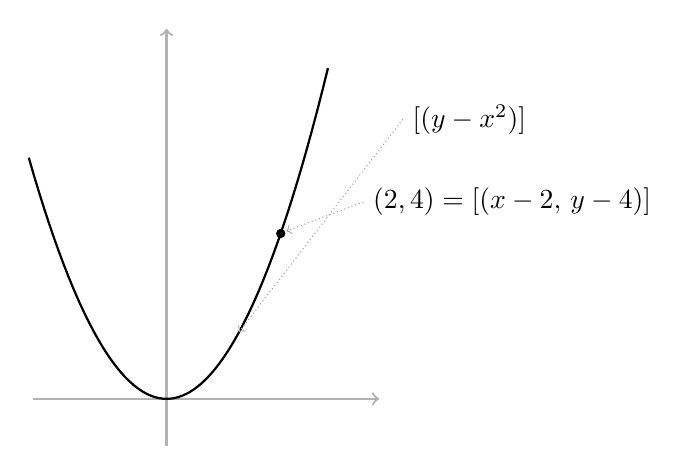
\begin{tikzpicture}[scale=1.0]
  \draw[gray!60,thick,->] (-1.7,0) -- (2.7,0);
  \draw[gray!60,thick,->] (0,-0.6) -- (0,4.7);
  \draw[thick] plot[domain=-1.75:2.05,samples=61] ({\x},{\x*\x});
  \fill (1.45,2.1) circle (1.7pt);
  \node[anchor=west] (genlab) at (3.0,3.55) {$[(y-x^2)]$};
  \draw[gray!70,densely dotted,->] (genlab.west) -- (0.92,0.85);
  \node[anchor=west] (speclab) at (2.5,2.5) {$(2,4)=[(x-2,\,y-4)]$};
  \draw[gray!70,densely dotted,->] (speclab.west) -- (1.52,2.13);
\end{tikzpicture}
\caption{$(2,4)=[(x-2,\,y-4)]$ 是 $[(y-x^2)]$ 的一个\trSpecialization{}；$[(y-x^2)]$ 是 $(2,4)$ 的一个\trGenerization{}。（依原书手绘图重绘。）}\label{fig:specialization-generization}
\end{figure}

\begin{exercise}\label{ex:specialization-primes}
设 $X=\Spec A$，证明：$[\mathfrak{q}]$ 是 $[\mathfrak{p}]$ 的一个\trSpecialization{}，当且仅当 $\mathfrak{p}\subset\mathfrak{q}$。进而证明 $V(\mathfrak{p})=\overline{\{[\mathfrak{p}]\}}$。
\end{exercise}

\textbf{3.6.11.}\ \emph{\trhDefinition{}。}\quad 设 $K$ 是一个\trClosedSubset。若 $\overline{\{p\}}=K$，就称\trTopologicalSpace{}的点 $p\in X$ 是 $K$ 的一个\textbf{\trGenericPoint}（generic point）。

这个重要概念早于\trGrothendieck{}而存在。二十世纪初的意大利代数几何学派对簇的「\trGenericPoint」已有一个概念：他们指的是不带任何特殊性质的点，于是凡对「一个\trGenericPoint」证明了的命题，对簇上「几乎所有」的点都真。现代的「\trGenericPoint」有着同样的直观含义。如果某件事对不可约子集的诸点「泛性地」或「大体地」成立——即对某个\trDense{}\trOpenSubset（对应「几乎所有的点」）成立——那么它对\trGenericPoint{}成立，反之亦然。（这是一条原理性的陈述，而非事实陈述。一个有趣的情形是「既约性」：这条原理对一般的概形并不成立，但对诸如簇这样「合理」的概形则\emph{确实}成立；参看注记~5.2.2。）例如，一个函数在不可约概形的\trGenericPoint{}处取值为零，当且仅当它在所有点处都取值为零。请留心这类其他例子。

\textbf{\trGeneralPoint{}}（general point）这个词的含义则不同。「$X$ 的\trGeneralPoint{}满足如此这般的性质」这句话，意思是「$X$ 的某个\trDense{}\trOpenSubset{}的每个点都满足如此这般的性质」。当心不要混淆「泛」与「一般」。但要警惕：公认的术语并不总遵循这条约定；「一般光滑性」（\S21.6.3）与「一般平坦性」（定理~24.5.13）便是明证。\footnote{译注：为与「一般点」（generic point，见\trGenericPoint）相区分，本译本把 general point 固定译作「\trGeneralPoint{}」。}

\begin{exercise}\label{ex:generic-point-parabola}
验证 $[(y-x^2)]\in\mathbb{A}^2_{\mathbb{C}}$ 是 $V(y-x^2)$ 的一个\trGenericPoint。
\end{exercise}

再给「一般」这个术语一点动机：我们把 $[(y-x^2)]$ 想成抛物线上某个不特定的点（而闭点 $(a,a^2)\in\mathbb{C}^2$，即 $(x-a,\,y-a^2)$（其中 $a\in\mathbb{C}$），则是「特定的点」）；按这个词的日常用法，它也是「一般的」。我们可以把它「\trSpecialization{}」到抛物线的某个特定的点；于是例如，$(2,4)$ 就是 $[(y-x^2)]$ 的一个\trSpecialization{}。（再一次，见图~\ref{fig:specialization-generization}。）为把这件事讲得更精确些：

\begin{exercise}[容易的练习]\label{ex:generic-point-near-every-point}
设 $\mathfrak{p}$ 是\trClosedSubset{} $K$ 的一个\trGenericPoint。证明它「邻近 $K$ 的每个点 $\mathfrak{q}$」（$\mathfrak{q}$ 的每个\trNeighborhood{}都含有 $\mathfrak{p}$），并且「不邻近任何不在 $K$ 中的点 $\mathfrak{r}$」（存在 $\mathfrak{r}$ 的一个不含 $\mathfrak{p}$ 的\trNeighborhood）。（这一想法曾在 \S3.2.4 例~1 与\cref{ex:topological-space-a1k} 中出现过。）
\end{exercise}

我们很快就会看到（练习~3.7.F）：$\Spec A$ 的点与 $\Spec A$ 的不可约闭子集之间有一个自然双射，它把每个点送到其闭包，把每个不可约闭子集送到它的（唯一的）\trGenericPoint。你现在就可以证明这件事，但我们想等发展出一些便利的术语再说。

\textbf{3.6.12.\ \trIrreducibleComponent{}、\trConnectedComponent{}，以及诸\trNoetherian{}条件。}\quad \trTopologicalSpace{}的一个\textbf{\trIrreducibleComponent{}}（irreducible component）是一个极大的\trIrreducible{}子集（即不被任何更大的\trIrreducible{}子集包含的\trIrreducible{}子集）。\trIrreducibleComponent{}都是闭的（因为\trIrreducible{}子集的闭包仍\trIrreducible，\cref{ex:irreducible-open-dense}(b)），而且把\trTopologicalSpace{} $X$ 的\trIrreducibleComponent{}想成 $X$ 的诸\trIrreducible{} \emph{闭}子集中的极大者，会有帮助。我们把它们看作「$X$ 的诸块」（见图~\ref{fig:irreducible-components}）。

\begin{figure}[htbp]
\centering
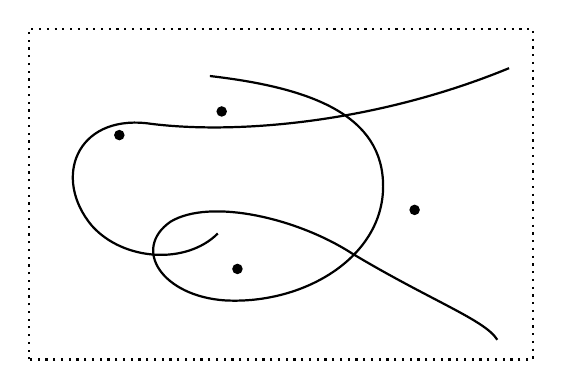
\begin{tikzpicture}[scale=1.0]
  \draw[dotted,thick] (-3.2,-2.1) rectangle (3.2,2.1);
  \draw[thick] (2.9,1.6) .. controls (1.2,0.9) and (-0.6,0.75) .. (-1.7,0.9)
    .. controls (-2.6,1.0) and (-2.9,0.2) .. (-2.4,-0.4)
    .. controls (-2.0,-0.85) and (-1.2,-0.9) .. (-0.8,-0.5);
  \draw[thick] (-0.9,1.5) .. controls (0.4,1.35) and (1.3,1.0) .. (1.3,0.1)
    .. controls (1.3,-0.8) and (0.3,-1.4) .. (-0.7,-1.35)
    .. controls (-1.5,-1.3) and (-1.9,-0.7) .. (-1.4,-0.35)
    .. controls (-0.9,-0.05) and (0.2,-0.3) .. (0.9,-0.75)
    .. controls (1.9,-1.35) and (2.6,-1.6) .. (2.75,-1.85);
  \fill (-2.05,0.75) circle (1.9pt);
  \fill (-0.75,1.05) circle (1.9pt);
  \fill (-0.55,-0.95) circle (1.9pt);
  \fill (1.7,-0.2) circle (1.9pt);
\end{tikzpicture}
\caption{$\mathbb{A}^2_{\mathbb{C}}$ 的这个\trClosedSubset{}有六个\trIrreducibleComponent{}。（依原书手绘图重绘。）}\label{fig:irreducible-components}
\end{figure}

类似地，\trTopologicalSpace{} $X$ 的子集 $Y$ 若是极大的\trConnected{}子集（即不被任何更大的\trConnected{}子集包含的\trConnected{}子集），就称为一个\textbf{\trConnectedComponent{}}（connected component）。

\begin{exercise}[每个\trTopologicalSpace{}都是诸\trIrreducibleComponent{}之并]\label{ex:point-in-irreducible-component}
证明\trTopologicalSpace{} $X$ 的每个点 $p$ 都含于 $X$ 的某个\trIrreducibleComponent{}。提示：\trZornsLemma。更精确地说，考虑由 $X$ 的含 $p$ 的诸\trIrreducible{}子集所组成的\trPoset{} $\scr S$。证明 $\scr S$ 存在极大的全序子集 $\{Z_\alpha\}$。证明 $\bigcup Z_\alpha$ 是\trIrreducible{}的。
\end{exercise}

\textbf{3.6.13.}\ \emph{\trhRemark{}。}\quad 每个点都含于某个\trConnectedComponent{}，而\trConnectedComponent{}总是闭的。你现在就可以证明这件事，但我们刻意把它推迟到需要它之时，那是一个带星的选学小节（练习~10.5.J）。另一方面，\trConnectedComponent{}未必是开的；参看 [Stacks, tag 004T]。\trConnectedComponent{}不是开集的\trAffineScheme{}的一个例子是 $\Spec\bigl(\prod_i^{\infty}\mathbb{F}_2\bigr)$。

\textbf{3.6.14.}\quad 在我们考虑过的诸例中，这些空间都自然地分裂成有限多个\trIrreducibleComponent{}。例如，$\mathbb{A}^2_k$ 中 $xy=0$ 的\trLocus，我们把它想成有两「块」——两条坐标轴。原因在于：它们的底\trTopologicalSpace（我们很快将予确立）是\textbf{\trNoetherian}（Noetherian）的。若\trTopologicalSpace{} $X$ 对\trClosedSubset{}满足\textbf{\trDescendingChainCondition{}}（descending chain condition）：任何一列\trClosedSubset{} $Z_1\supset Z_2\supset\cdots\supset Z_n\supset\cdots$ 都终将稳定下来——存在 $r$ 使得 $Z_r=Z_{r+1}=\cdots$——就称 $X$ 是\trNoetherian{}的。这里给出第一个例子（你应当不用\trNoetherian{}环而把它显式做出来）。

\begin{exercise}\label{ex:a2-noetherian}
证明 $\mathbb{A}^2_{\mathbb{C}}$ 是\trNoetherian{}\trTopologicalSpace：$\mathbb{A}^2_{\mathbb{C}}=\Spec\mathbb{C}[x,y]$ 的任何一列递减的\trClosedSubset{}都必终将稳定。注意稳定所需的时长可以任意长。（$\mathbb{A}^2_{\mathbb{C}}$ 的诸\trClosedSubset{}已在 \S3.4.5 中描述过。）证明：带\trClassicalTopology{}的 $\mathbb{C}^2$ \emph{不是}\trNoetherian{}\trTopologicalSpace。
\end{exercise}

\textbf{3.6.15.}\ \textbf{\trhProposition{}。}\ ——\ \emph{设 $X$ 是\trNoetherian{}\trTopologicalSpace。则每个非空\trClosedSubset{} $Z$ 都能唯一地表示成有限并 $Z=Z_1\cup\cdots\cup Z_n$，其中诸 $Z_i$ 是\trIrreducible{}的\trClosedSubset，且没有一个包含于另一个之中。}

翻译一下：任何\trClosedSubset{} $Z$ 都只有有限多个「块」。

\emph{证明。}\quad 下述技术称为\textbf{诺特归纳}（Noetherian induction），理由将会明朗。我们还会多次使用它。考虑 $X$ 的那些\emph{不能}表示成不可约闭子集之有限并的非空\trClosedSubset{}所成的族。我们来证明这个族是空的。否则，设 $Y_1$ 是其中一个。若 $Y_1$ 真包含另一个这样的成员，就选一个，称为 $Y_2$。若 $Y_2$ 又真包含另一个这样的成员，就选一个，称为 $Y_3$，如此等等。由\trDescendingChainCondition{}，这个过程必终将停止，于是我们有某个 $Y_r$，它不能写成不可约闭子集的有限并，但真包含于它的每个\trClosedSubset{}却都能这样写。然而 $Y_r$ 自身并不可约，故可写 $Y_r=Y'\cup Y''$，其中 $Y'$ 与 $Y''$ 都是真\trClosedSubset。由假设，这两者都能写成有限多个不可约闭子集之并，于是 $Y_r$ 也能，矛盾。这样一来，每个\trClosedSubset{}都能写成不可约闭子集的有限并。通过丢弃其中若干个，不妨设这些不可约闭子集互不包含。

我们接着证唯一性。设
\[
Z=Z_1\cup Z_2\cup\cdots\cup Z_r=Z'_1\cup Z'_2\cup\cdots\cup Z'_s
\]
是两种这样的表示。则 $Z'_1\subset Z_1\cup Z_2\cup\cdots\cup Z_r$，于是 $Z'_1=(Z_1\cap Z'_1)\cup\cdots\cup(Z_r\cap Z'_1)$。现在 $Z'_1$ 是\trIrreducible{}的，故这些成员之一就是 $Z'_1$ 本身，比如说（不失一般性）$Z_1\cap Z'_1$。于是 $Z'_1\subset Z_1$。类似地，$Z_1\subset Z'_\alpha$ 对某个 $\alpha$ 成立；但由于 $Z'_1\subset Z_1\subset Z'_\alpha$，而 $Z'_1$ 不含于其他任何 $Z'_j$，必有 $\alpha=1$，从而 $Z'_1=Z_1$。这样，$Z$-名单中的每个成员都在 $Z'$-名单中，反之亦然，所以两张名单必是同一张。\hfill$\square$

\begin{exercise}\label{ex:connected-components-union-irreducible}
证明\trTopologicalSpace{} $X$ 的每个\trConnectedComponent{}都是 $X$ 的若干\trIrreducibleComponent{}之并。证明：$X$ 的任何同时开且闭的子集必是 $X$ 的某几个\trConnectedComponent{}之并。设 $X$ 是\emph{\trNoetherian}的\trTopologicalSpace，证明：$X$ 的任意一组\trConnectedComponent{}之并总是在 $X$ 中既开又闭。（特别地，\trNoetherian{}\trTopologicalSpace{}的\trConnectedComponent{}总是开的；这对更一般的\trTopologicalSpace{}并不成立，参看注记~3.6.13。）
\end{exercise}

\textbf{3.6.16.\ \trNoether{}环。}\quad 事实证明，我们考虑过的全部谱（带星的\cref{ex:spec-quasicompact}(b) 除外）都是\trNoetherian{}\trTopologicalSpace，但这并非对一切环的谱都成立。我们的例子所共有的关键特征是：这些环都是\emph{\trNoetherian}的。若一个\trRing{}的诸\trIdeal{}的每个升链 $I_1\subset I_2\subset\cdots$ 都终将稳定：存在 $r$ 使得 $I_r=I_{r+1}=\cdots$，就称它是\textbf{\trNoetherian}的。（这对\trIdeal{}而言称为\textbf{\trAscendingChainCondition{}}（ascending chain condition）。）

下面是关于\trNoetherian{}环的几条速记事实。你应当能把它们全部证明：
\begin{itemize}
\item \trField{}都是\trNoetherian{}的。$\mathbb{Z}$ 是\trNoetherian{}的。
\item （\trNoetherian{}性在取商下保持。）若 $A$ 是\trNoetherian{}的，$I$ 是 $A$ 的任一\trIdeal，则 $A/I$ 是\trNoetherian{}的。
\item （\trNoetherian{}性在\trLocalization{}下保持。）若 $A$ 是\trNoetherian{}的，$S$ 是任一\trMultiplicativeSubset，则 $S^{-1}A$ 是\trNoetherian{}的。
\end{itemize}

\begin{exercise}\label{ex:pid-noetherian}
证明\trPID{}都是\trNoetherian{}环。
\end{exercise}

\begin{exercise}[重要练习]\label{ex:noetherian-finitely-generated-ideals}
证明：\trRing{} $A$ 是\trNoetherian{}的，当且仅当 $A$ 的每个\trIdeal{}都是\trFinitelyGenerated{}的。
\end{exercise}

下一条事实就不平凡了。

\textbf{3.6.17.\ \trHilbert{}基定理。}\ ——\ \emph{若 $A$ 是\trNoetherian{}的，则 $A[x]$ 亦然。}

\trHilbert{}在划时代的论文 [Hil] 中证明了这个定理；他还在同一篇论文中证明了\trHilbert{}合冲定理（\S16.1.2），并定义了\trHilbert{}函数，证明它们最终成为多项式（\S18.6）。

\textbf{3.6.18.}\quad 由上述结果，任意域上的、或者整数环上的有限多元多项式环都是\trNoetherian{}的——其任何商或局部化亦然。于是例如，$k$ 或 $\mathbb{Z}$ 上任何有限生成的代数，以及其任何局部化，都是\trNoetherian{}的。大多数「好」环都是\trNoetherian{}的，但并非所有的环都\trNoetherian：$k[x_1,x_2,\dots]$ 就不是，因为 $(x_1)\subset(x_1,x_2)\subset(x_1,x_2,x_3)\subset\cdots$ 是\trIdeal{}的一条严格升链（参看\cref{ex:spec-quasicompact}(b)）。

\textbf{3.6.19.}\ \emph{\trHilbert{}基定理 3.6.17 的证明。}\quad 我们来证明\trIdeal{} $I\subset A[x]$ 都是\trFinitelyGenerated{}的。我们归纳地构造一组生成元 $f_1,\dots$，方法如下。对 $n\ge 0$，若 $I\neq(f_1,\dots,f_n)$，就取 $f_{n+1}$ 为 $I-(f_1,\dots,f_n)$ 中次数最低的任一非零元素。于是（假定 $I\neq(0)$）$f_1$ 就是 $I$ 中次数最低的任一元素。若这个程序终止，我们就完成了。否则，令 $a_n\in A$ 为 $f_n$ 的最低次项系数（对一切 $n>0$）。由于 $A$ 是\trNoetherian{}的，存在 $N$ 使得 $(a_1,a_2,\dots)=(a_1,\dots,a_N)$。设 $a_{N+1}=\sum_{i=1}^{N}b_ia_i$。那么
\[
f_{N+1}-\sum_{i=1}^{N}b_if_ix^{\deg f_{N+1}-\deg f_i}
\]
是 $I$ 中一个不属于 $(f_1,\dots,f_N)$ 的元素（因为 $f_{N+1}\notin(f_1,\dots,f_N)$），并且次数低于 $f_{N+1}$，这与我们本应选取 $f_{N+1}$ 的方式相矛盾。\hfill$\square$

现在我们把\trNoetherian{}环与\trNoetherian{}\trTopologicalSpace{}联系起来。

\begin{exercise}\label{ex:noetherian-ring-spec-noetherian}
设 $A$ 是\trNoetherian{}的，证明 $\Spec A$ 是\trNoetherian{}\trTopologicalSpace。描述一个\trRing{} $A$，使得 $\Spec A$ 不是\trNoetherian{}\trTopologicalSpace。（题外话：若 $\Spec A$ 是\trNoetherian{}\trTopologicalSpace，$A$ 未必\trNoetherian。一个例子是 $A=k[x_1,x_2,x_3,\dots]/(x_1,\,x_2^2,\,x_3^3,\dots)$。此时 $\Spec A$ 只有一个点，因而是\trNoetherian{}的。但 $A$ 不是\trNoetherian{}的，因为在 $A$ 中 $(x_1)\subsetneq(x_1,x_2)\subsetneq(x_1,x_2,x_3)\subsetneq\cdots$。）
\end{exercise}

\begin{exercise}[练习~3.6.G(b) 所许诺的]\label{ex:noetherian-open-quasicompact}
证明\trNoetherian{}\trTopologicalSpace{}的每个\trOpenSubset{}都是\trQuasicompact{}的。于是若 $A$ 是\trNoetherian{}的，$\Spec A$ 的每个\trOpenSubset{}都是\trQuasicompact{}的。（如果你愿意，也可以对带诱导拓扑的\emph{任何}子集证明这个结果。）
\end{exercise}

\textbf{3.6.20.\ 留供后用：模的\trNoetherian{}条件。}\quad 一个重要的相关概念是\trNoetherian{}\emph{模}。虽然我们要过一阵子才会用到这个概念（\S10.7.3），但我们打算趁\trNoetherian{}观念在你脑海中还新鲜之时，发展其最重要的性质。设 $A$ 是任一\trRing，不必\trNoetherian。若一个 $A$-模对子模满足\trAscendingChainCondition{}，就称这个 $A$-模是\textbf{\trNoetherian}的（Noetherian $A$-module）。于是例如：\trRing{} $A$ 是\trNoetherian{}的，当且仅当它作为 $A$-模是\trNoetherian{}的。

\begin{exercise}[参看重要的\cref{ex:noetherian-finitely-generated-ideals}]\label{ex:noetherian-module-submodule-fg}
证明：若 $M$ 是\trNoetherian{} $A$-模，则 $M$ 的任何子模都是\trFinitelyGenerated{}的 $A$-模。（事实上逆命题也真，你尽管把它也证了。）
\end{exercise}

\begin{exercise}\label{ex:noetherian-module-extension}
若 $0\to M'\to M\to M''\to 0$ 是\trExactSequence，证明：$M'$ 与 $M''$ 是\trNoetherian{}的，当且仅当 $M$ 是\trNoetherian{}的。（提示：给定 $M$ 中的一条升链，我们在 $M'$ 与 $M''$ 中得到两条同步的升链。可能的进一步提示：证明：若
\[
M'\longrightarrow M\xrightarrow{\ \phi\ }M''
\]
是\trExactSequence，$N\subset N'\subset M$，且 $N\cap M'=N'\cap M'$、$\phi(N)=\phi(N')$，则 $N=N'$。）
\end{exercise}

\begin{exercise}\label{ex:noetherian-free-module}
证明：若 $A$ 是\trNoetherian{}环，则 $A^{\oplus n}$ 是\trNoetherian{} $A$-模。
\end{exercise}

\begin{exercise}\label{ex:finitely-generated-noetherian-module}
证明：若 $A$ 是\trNoetherian{}环，$M$ 是有限生成的 $A$-模，则 $M$ 是\trNoetherian{}模。于是由\cref{ex:noetherian-module-submodule-fg}：\trNoetherian{}环上有限生成模的任何子模都是有限生成的。
\end{exercise}

\textbf{3.6.21.\ 你为什么不必为\trNoetherian{}假设操心。}\quad 你该不该辛辛苦苦去消除\trNoetherian{}假设？你该不该为\trNoetherian{}假设操心？你该不该夜里睡不着觉、满脑子想着非\trNoetherian{}环？对大多数人来说，这些问题的答案是「不必」。多数人永远不需要为非\trNoetherian{}环操心，但也有理由对它们持开放态度。首先，它们真的会冒出来。例如，\trNoetherian{}\trScheme{}在\trNoetherian{}\trScheme{}上的\trFiberProduct（甚至连\trNoetherian{}点在\trNoetherian{}点上的\trFiberProduct！）可以是非\trNoetherian{}的（警告~10.1.5），而\trNoetherian{}环的\trNormalization{}也可以是非\trNoetherian{}的（警告~10.7.4）。你可以辛苦地去证明你关心的那些环或概形没有这种病态，也可以索性放松，不去操心它。其次，一般地与概形打交道往往并无害处。知道何时需要\trNoetherian{}条件，会帮你记住结果为何为真，因为你会对\trNoetherian{}条件从何处进入论证有某种感觉。最后，对某些人来说，非\trNoetherian{}环会自然出现。例如，阿代尔（ad\`ele）不是\trNoetherian{}的。而算术与热带几何中自然出现的许多\trValuationRing{}（valuation ring）也都不是\trNoetherian{}的。
